% !TEX root = ../ClassicThesis_DEIB.tex

\chapter{The Robì project} \label{chap:robìProject}

A branch of this thesis work involved the customization of the prototype mobile manipulator Robì \parencite{robi} to the requirements of the mobile base requested by the \ac{GRAPE} project. 


\begin{figure}
	\centering
	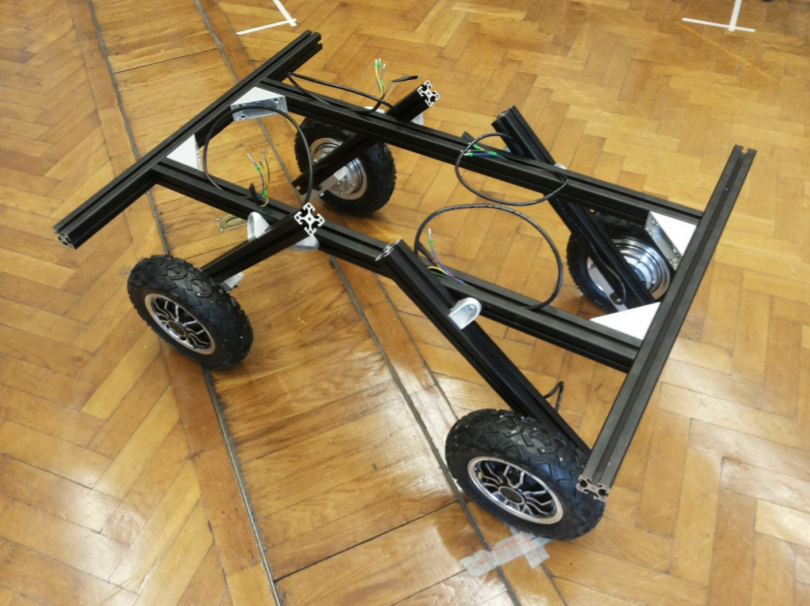
\includegraphics[width=0.6\textwidth]{Images/robi/robi_inizio.png}
	\caption{\textit{The Robì mobile manipulator chassis, in one of its}}
	\label{fig:robiDefault}
\end{figure}


\section{Robì mobile manipulator}
Robì (see Figure \ref{fig:robiDefault}) is a prototype small-sized mobile manipulator for agricultural applications, whose aim is to support the development and testing of innovative perception and control algorithms. Both the mechanical structure and the motion control system are designed to be simple, flexible, low-cost and low-weight, to create a system that can act as an open source base for project in agricultural robotics.
Since the platform is thought as a versatile mobile base to be adapted to several fields (\textit{e.g.} vineyards, herbaceous plants) its chassis is designed to have flexible geometrical characteristics (ground clearance, track, wheelbase) in the ranges explained in Table \ref{tab:robiConfiguration}. 

 \begin{table}[tb]
\footnotesize
\centering
\begin{tabularx}{0.45\textwidth}{ll}
\toprule
\tablefirstcol{l}{Ground clearance}
& [0.25, 0.35] m \\
\tablefirstcol{l}{Track}
& [0.75, 1.2] m \\
\tablefirstcol{l}{Wheelbase}
& [0.6, 1] m \\
\toprule
\end{tabularx}
\caption[Process point cloud action specification]{Process point cloud action specification}
\label{tab:robiConfiguration}
\end{table}


In Figure \ref{fig:robiConfigurations}
 More generally, the design of Robì aims to the principles of:
 
\begin{itemize}
	\item \textbf{low cost}, to make it easier to use it for example applications and, possibly, fleet-based applications
	\item \textbf{low weight}, to increase the battery life and, consequently, allow for more long and versatile missions
	\item \textbf{simple mechanical design}, to make it easy to build it out of a mounting kit
\end{itemize}

\begin{figure}
	\centering
	\subfloat[]{%
		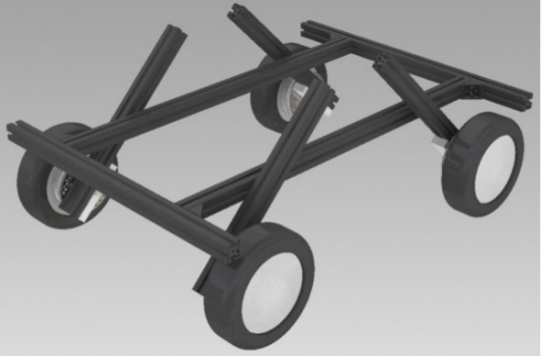
\includegraphics[width=0.45\textwidth]{Images/robi/robi_config1.png}
		\label{fig:robiConfig1}}
	\qquad
	\subfloat[]{%
		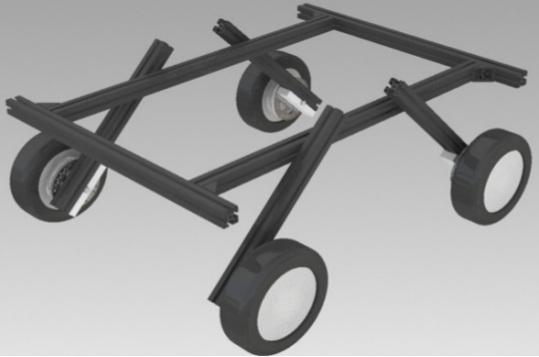
\includegraphics[width=0.45\textwidth]{Images/robi/robi_config2.png}
		\label{fig:robiConfig2}} \\
	\subfloat[]{%
		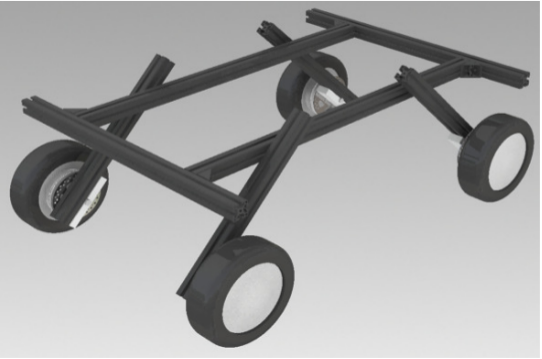
\includegraphics[width=0.45\textwidth]{Images/robi/robi_config3.png}
		\label{fig:robiConfig3}}
	\caption{\textit{3D rendering of different configuration of Robì base, obtained thanks to the chassis mechanical design.}}
	\label{fig:robiConfigurations}
\end{figure}




\begin{itemize}
	\item obiettivo: realizzare un'altra base mobile alternativa all'husky su cui portare il sistema GRAPE
	\item architettura hw: sensori che ci sono montati a bordo, spiegazione sistema controllo motori tramite CAN usando la board STM
	\item architettura sw: compatibile con quella di Grape, a meno dei nodi driver dei sensori e attuatori
	\item spiegazioni e immagini del vario hardware
\end{itemize}
